\chapter{Phá vỡ siêu đối xứng tự phát và đa bội \texorpdfstring{\(SU(5)\)}{SU(5)} đầu tiên}

\lectureoverview{Sự phá vỡ đối xứng trước hết xuất hiện ở đây như một sự kiện nhìn thấy được của phổ: một nguyên tử bất biến quay có các mức xung lượng góc suy biến, còn từ trường thì tách chúng ra. Một nam châm sắt sau đó cho thấy bài học tinh tế hơn rằng các phương trình có thể vẫn giữ một đối xứng mà chân không thì không. Magnon không khe, điều kiện \(J|0\rangle\neq0\), và một tham số trật tự khác không là ba mô tả của cùng hiện tượng ấy. Chúng ta mang khuôn mẫu này vào một lý thuyết trường siêu đối xứng chiral, suy ra thế vô hướng \(V=|W'|^2\) bằng cách khử trường phụ trợ \(F\), và phân biệt các chân không siêu đối xứng với các chân không phá vỡ \(F\). Năng lượng chân không thu được, sự tách boson--fermion, goldstino, sector ẩn, và cơ chế siêu-Higgs hoàn tất phần thảo luận về siêu đối xứng. Phần cuối đổi chủ đề và mở đầu thống nhất lớn: \(SU(3)\times SU(2)\times U(1)\) được nhúng theo từng khối vào \(SU(5)\), mà đa bội vật chất đầu tiên của nó kết hợp một bộ đôi lepton với ba phản quark down.}

\section{Phổ ghi nhớ đối xứng của nó}

Mục đích của việc bắt đầu bằng một nguyên tử không chỉ đơn thuần là ôn lại cơ học lượng tử sơ cấp. Các mức năng lượng và khối lượng hạt là cùng một loại dữ liệu phổ. Nếu một đối xứng buộc các mức nguyên tử trùng nhau, thì sự phá vỡ của nó có thể tách những mức ấy; trong lý thuyết trường, phát biểu tương ứng là các thành viên của một đa bội hạt có thể nhận những khối lượng khác nhau.

Hãy xét một trạng thái nguyên tử có tổng xung lượng góc \(j\), bao gồm cả đóng góp spin lẫn quỹ đạo. So với bất kỳ trục nào được chọn,
\begin{equation}
J_z|j,m\rangle=m\hbar|j,m\rangle,
\qquad
m=-j,-j+1,\ldots,j,
\end{equation}
vì vậy có \(2j+1\) trạng thái. Không nên hiểu các mũi tên quen thuộc trong giáo trình như thể vectơ xung lượng góc theo nghĩa đen chỉ có \(2j+1\) hướng không gian khả dĩ. Thứ bị lượng tử hóa là thành phần của nó dọc theo trục đã chọn.

Trong không gian trống, bất biến đối với phép quay, không có lý do vật lý nào để ưu tiên trục đó. Một phép quay trộn các trạng thái trong đa bội spin-\(j\), và tính bất biến của Hamiltonian hàm ý
\begin{equation}
[H,\mathbf J]=0,
\qquad
E_{j,-j}=E_{j,-j+1}=\cdots=E_{j,j}.
\label{eq:l9-degeneracy}
\end{equation}

\begin{classroomqa}
\audiencequestion{Đối xứng nào nói rằng quay toàn bộ nguyên tử không thể làm thay đổi năng lượng của nó? \lecturetimestamp{00:05:53}}
\lecturerresponse{Đối xứng quay. Vì một phép quay đưa một định hướng của xung lượng góc sang một định hướng khác mà không làm thay đổi hệ vật lý, nên mọi trạng thái \(2j+1\) đều có cùng năng lượng.}
\end{classroomqa}

Bây giờ đặt một từ trường \(\mathbf B=B\hat{\mathbf z}\). Tương tác
\begin{equation}
H_B=-\boldsymbol{\mu}\cdot\mathbf B
\end{equation}
phân biệt thành phần song song với từ trường. Một cách sơ đồ,
\begin{equation}
\Delta E_m\propto mB.
\label{eq:l9-zeeman}
\end{equation}
Các mức có \(m\) khác nhau tách ra tuyến tính ở từ trường yếu, và các chuyển tiếp giữa chúng làm tách các vạch phổ.

\begin{classroomqa}
\audiencequestion{Sự tách các mức nguyên tử trong từ trường được gọi là gì? \lecturetimestamp{00:07:13}}
\lecturerresponse{Hiệu ứng Zeeman. Đó là nguyên mẫu cho toàn bộ phần thảo luận: các mức trở nên suy biến do một đối xứng sẽ tách ra khi một nền phá vỡ đối xứng ấy.}
\end{classroomqa}

\begin{center}
\begin{tikzpicture}[x=1.05cm,y=0.75cm,>=Latex]
  \draw[thick] (-3,0) -- (-1,0);
  \node[left] at (-3,0) {\(B=0\)};
  \foreach \y/\m in {-1.2/-1,-0.4/0,0.4/1,1.2/2} {
    \draw[thick,teal!70!black] (1,\y) -- (3,\y);
    \node[right] at (3,\y) {\(m=\m\)};
  }
  \draw[->,thick] (-0.5,0) -- (0.6,0);
  \node[above] at (0.05,0) {\(\mathbf B\neq0\)};
\end{tikzpicture}
\end{center}

\section{Chất sắt từ: các định luật đối xứng, chân không bất đối xứng}

Một bức tranh vi mô đơn giản của nam châm sắt gán cho mỗi vị trí một moment từ nhỏ. Nếu các moment lân cận hạ thấp năng lượng của chúng bằng cách trở nên song song, thì pha nhiệt độ thấp là sắt từ. Nếu sự sắp hàng phản song song được ưa chuộng, kết quả là phản sắt từ. Dao động nhiệt hoặc lượng tử mạnh thay vào đó có thể xóa sạch mọi từ hóa thuần.

Giả sử một nam châm sắt chiếm đầy thế giới và ổn định vào một trạng thái thẳng hàng đồng đều. Từ trường nội tại của nó tách các mức của một nguyên tử hệt như một trường áp đặt từ bên ngoài. Tuy vậy, có một khác biệt mang tính quyết định. Các tương tác nền tảng không ưu tiên hướng bắc, hướng đông, hay bất kỳ hướng nào khác. Mọi cấu hình quay đồng đều đều có cùng năng lượng:
\begin{equation}
\mathbf M(\mathbf x)=M_0\hat{\mathbf n},
\qquad
\hat{\mathbf n}\in S^2.
\label{eq:l9-ferromagnetic-vacua}
\end{equation}
Các phương trình là bất biến quay, nhưng một trạng thái cơ bản thực sự lại chọn một \(\hat{\mathbf n}\). Đây là sự phá vỡ đối xứng tự phát chứ không phải hiển minh.

Một cư dân được tạo nên từ các kích thích của môi trường này không thể nắm lấy toàn bộ vũ trụ rồi quay nó đi. Vì thế, về cục bộ, hướng đã được chọn trông cơ bản chẳng khác gì một từ trường ngoài. Một nguyên tử vẫn thấy cùng mẫu mức đó, với xung lượng góc của nó được phân giải dọc theo \(\hat{\mathbf n}\) thay vì dọc theo trục \(z\) được đặt tên từ bên ngoài. Câu hỏi là một quan sát viên nội tại có thể phát hiện thế nào rằng sự bất đối xứng bề ngoài thuộc về trạng thái chứ không thuộc về các định luật.

\subsection{Dấu hiệu Goldstone}

Một phép quay đồng đều của mọi moment chuyển từ một chân không trong ~\eqref{eq:l9-ferromagnetic-vacua} sang một chân không khác và không tốn năng lượng. Thay vào đó, hãy để định hướng biến thiên rất từ từ theo không gian. Khi ấy các moment lân cận kéo lẫn nhau và sự méo lan truyền như một sóng spin, mà các lượng tử của nó là magnon. Khi bước sóng tiến tới vô hạn, cấu hình tiến gần tới một phép quay đồng đều, nên năng lượng kích thích của nó tiến tới không:
\begin{equation}
k=\frac{2\pi}{\lambda}\longrightarrow0
\quad\Longrightarrow\quad
E(k)\longrightarrow0.
\label{eq:l9-gapless-magnon}
\end{equation}
Hai cư dân có thể làm dao động các moment lân cận, gửi những sóng như thế qua môi trường, và đo năng lượng nhỏ tùy ý này. Thí nghiệm đó bộc lộ sự phá vỡ tự phát dù họ không thể quay cả thế giới.

\editorialnote{Một magnon sắt từ là không khe nhưng nhìn chung có quan hệ tán sắc bậc hai phi tương đối tính \(E\propto k^2\), thay vì quan hệ tương đối tính \(E\propto|k|\). Bài giảng dùng từ không khối lượng theo nghĩa vật lý thích hợp là khe triệt tiêu. Cả hai đều là các mode Goldstone.}

Ý tưởng tương tự áp dụng cho các đối xứng nội liên tục, bao gồm các nhóm gauge và hương vị của vật lý hạt. Tuy nhiên, khi đối xứng bị phá vỡ là một đối xứng gauge, mode Goldstone không còn tồn tại như một hạt không khối lượng độc lập.

\begin{classroomqa}
\audiencequestion{Điều gì xảy ra khi sự phá vỡ đối xứng tự phát được kết hợp với tính bất biến gauge? \lecturetimestamp{00:15:56}}
\lecturerresponse{Boson Goldstone cung cấp một phân cực bổ sung cho trường gauge. Boson gauge trở nên có khối lượng; đó là cơ chế Higgs, mà ta sẽ quay lại trong phép tương tự hấp dẫn.}
\end{classroomqa}

\section{Ba dấu hiệu tương đương của sự phá vỡ}

Giờ đây nam châm sắt có thể được mô tả bằng ba cách diễn đạt bổ sung lẫn nhau.

\paragraph{Các chân không suy biến.}
Có một trạng thái năng lượng tối thiểu cho mỗi định hướng \(\hat{\mathbf n}\). Vật lý diễn ra trong một phần tử được chọn của họ này dù đối xứng liên hệ tất cả chúng với nhau.

\paragraph{Một bộ sinh không triệt tiêu chân không.}
Gọi \(J_a\) là một bộ sinh của các phép quay. Một phép biến đổi hữu hạn là
\begin{equation}
U(\epsilon)=e^{-i\epsilon J_a},
\end{equation}
và \(J_a|0\rangle\) tỉ lệ với biến thiên vô cùng bé của chân không, chứ không phải toàn bộ trạng thái đã quay.

\begin{classroomqa}
\audiencequestion{Các bộ sinh của đối xứng quay là gì? \lecturetimestamp{00:17:29}}
\lecturerresponse{Các thành phần của tổng xung lượng góc. Ta gọi chúng là \(J_a\) vì chúng quay mọi thứ trong trạng thái, chứ không chỉ một nguyên tử.}
\end{classroomqa}

Một bộ sinh không bị phá vỡ thỏa mãn
\begin{equation}
J_a|0\rangle=0.
\label{eq:l9-unbroken-generator}
\end{equation}
Thay vào đó, một bộ sinh bị phá vỡ cho
\begin{equation}
J_a|0\rangle\neq0.
\label{eq:l9-broken-generator}
\end{equation}

\begin{classroomqa}
\audiencequestion{Nếu \(J_a|0\rangle\) khác không, có phải nó đơn giản chỉ cho lại cùng chân không không? \lecturetimestamp{00:19:43}}
\lecturerresponse{Không. Nó cho hiệu vô cùng bé giữa chân không đã chọn và một chân không bị quay đi một chút. Về mặt vật lý, hiệu đó là một kích thích Goldstone có bước sóng vô hạn.}
\end{classroomqa}

\begin{classroomqa}
\audiencequestion{Phép quay vô cùng bé này có làm thay đổi năng lượng không? \lecturetimestamp{00:20:14}}
\lecturerresponse{Không. Chân không đã quay suy biến với chân không ban đầu, nên trạng thái Goldstone không xung lượng có năng lượng bằng không.}
\end{classroomqa}

Một cách ký hiệu,
\begin{equation}
J_a|0\rangle
\sim
|\pi_a,\mathbf k=0\rangle,
\label{eq:l9-generator-goldstone}
\end{equation}
trong đó \(\pi_a\) ký hiệu mode Goldstone gắn với bộ sinh bị phá vỡ.

\paragraph{Một tham số trật tự khác không.}
Từ hóa cục bộ \(\mathbf M(\mathbf x)\) là một trường. Trong pha nóng hoặc mất trật tự lượng tử,
\begin{equation}
\langle\mathbf M\rangle=0,
\end{equation}
và chân không không chọn một hướng nào. Trong pha có trật tự,
\begin{equation}
\langle M_i\rangle\neq0
\quad\text{for at least one component }i,
\label{eq:l9-magnetization-order}
\end{equation}
nên một phép quay trộn thành phần khác không đó vào các thành phần còn lại. Các chân không suy biến, một bộ sinh bị phá vỡ, và một tham số trật tự khác không là ba khuôn mẫu sẽ được mang sang siêu đối xứng.

\section{Nhắc lại bội chiral}

Ví dụ bốn chiều đơn giản nhất chứa một trường vô hướng phức, một fermion Weyl, và một trường vô hướng phức phụ trợ. Trong các tọa độ chiral,
\begin{equation}
y^\mu=x^\mu+i\bar\theta\bar\sigma^\mu\theta,
\end{equation}
một siêu trường chiral có thể được khai triển một cách sơ đồ thành
\begin{equation}
\Phi(y,\theta)=
\phi(y)+\sqrt2\,\theta\psi(y)+\theta^2F(y).
\label{eq:l9-chiral-expansion}
\end{equation}
Bài giảng lược bỏ hệ số quy ước \(\sqrt2\); từ đây chúng tôi đưa nó vào để các hệ số thành phần là chuẩn. Một siêu trường chiral vốn dĩ là phức: áp đặt tính thực không được bảo toàn dưới phép biến đổi siêu đối xứng của nó.

Tác dụng động học siêu đối xứng là
\begin{equation}
S_{\mathrm{kin}}
=
\int d^4x\,d^4\theta\,
\Phi^\dagger\Phi.
\label{eq:l9-kahler-action}
\end{equation}
Tích phân Grassmann chọn ra hệ số của
\(\theta^2\bar\theta^2\). Với metric mostly-minus, kết quả theo thành phần là
\begin{equation}
\mathcal L_{\mathrm{kin}}
=
\partial_\mu\phi^\ast\,\partial^\mu\phi
+i\bar\psi\bar\sigma^\mu\partial_\mu\psi
+F^\ast F.
\label{eq:l9-chiral-kinetic}
\end{equation}
Hai hạng đầu cho sự lan truyền của trường vô hướng và fermion. Hạng cuối không có đạo hàm và vì thế không lan truyền hạt nào.

\begin{figure}[H]
\centering
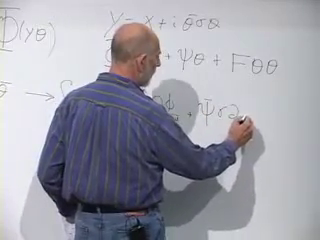
\includegraphics[width=0.76\textwidth]{lecture_09_figure_02.png}
\lectureframe{00:27:36.000}
\caption{Tọa độ chiral và khai triển theo thành phần; ở trên là các hạng vô hướng, fermion và phụ trợ.}
\end{figure}

\section{Tích phân \texorpdfstring{\(d^2\theta\)}{d2-theta} chọn ra điều gì}

Tương tác và khối lượng nảy sinh từ một hàm chỉnh hình \(W(\Phi)\), siêu thế:
\begin{equation}
S_W
=
\int d^4x
\left[
\int d^2\theta\,W(\Phi)
+\mathrm{h.c.}
\right].
\label{eq:l9-superpotential-action}
\end{equation}
Một biểu thức chiral không có sự phụ thuộc \(\bar\theta\) độc lập, nên nếu lấy tích phân của nó trên cả bốn tọa độ lẻ thì sẽ cho không. Thay vào đó, tích phân \(d^2\theta\) chọn ra thành phần \(\theta^2\) của nó.

Để thấy cách đếm tổ hợp trước khi xét một hàm tổng quát, lấy \(W(\Phi)=\Phi^n\). Trong
\begin{equation}
(\phi+\sqrt2\,\theta\psi+\theta^2F)^n,
\end{equation}
có hai cách để thu được đúng hai \(\theta\). Ta có thể chọn một \(F\theta^2\) duy nhất, hoặc chọn hai thừa số fermion.

\begin{classroomqa}
\audiencequestion{Có bao nhiêu hạng chứa một \(F\theta^2\) được chọn và ngoài ra chỉ có các vô hướng: \(n-1\) hay \(n\)? \lecturetimestamp{00:31:33}}
\lecturerresponse{Có \(n\). Bất kỳ một trong \(n\) thừa số nào cũng có thể cung cấp \(F\theta^2\); \(n-1\) thừa số còn lại cung cấp \(\phi\). Đóng góp là \(nF\phi^{n-1}\).}
\end{classroomqa}

\begin{classroomqa}
\audiencequestion{Có bao nhiêu cách để hai thừa số cung cấp hai fermion? \lecturetimestamp{00:32:26}}
\lecturerresponse{Có \(\binom n2=n(n-1)/2\) lựa chọn không có thứ tự. Phép co Grassmann cố định hạng \(\psi\psi\) tương ứng.}
\end{classroomqa}

Do đó, trong ký pháp lược bỏ hệ số của bài giảng,
\begin{equation}
\int d^2\theta\,\Phi^n+\mathrm{h.c.}
\;\leadsto\;
nF\phi^{n-1}
-\frac{n(n-1)}{2}\phi^{n-2}\psi\psi
+\mathrm{h.c.}
\label{eq:l9-power-extraction}
\end{equation}
Dấu trừ được viết ở đây tuân theo khai triển chuẩn hóa chuẩn và quy ước Grassmann; thay đổi quy ước có thể làm dịch chuyển những dấu bề ngoài.

\begin{classroomqa}
\audiencequestion{Điều gì đã xảy ra với hạng \(\phi^n\), hạng hoàn toàn không chứa \(\theta\) nào? \lecturetimestamp{00:33:10}}
\lecturerresponse{Nó có mặt trong tích, nhưng \(d^2\theta\) loại bỏ nó. Mũi tên có nghĩa là phép tích phân chọn hệ số \(\theta^2\); đó không phải là sự bằng nhau của toàn bộ các biểu thức.}
\end{classroomqa}

\begin{figure}[H]
\centering
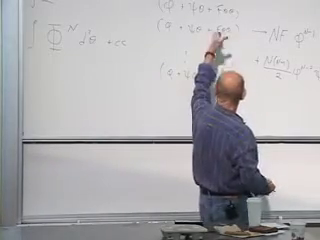
\includegraphics[width=0.82\textwidth]{lecture_09_figure_03.png}
\lectureframe{00:33:38.000}
\caption{Các thừa số siêu trường lặp lại và mũi tên kéo theo trích ra, chứ không phải đồng nhất với, thành phần hai-\(\theta\) của chúng.}
\end{figure}

Cộng các lũy thừa với những hệ số tùy ý biến các hệ số tổ hợp thành các đạo hàm:
\begin{equation}
\int d^2\theta\,W(\Phi)+\mathrm{h.c.}
\;\leadsto\;
F W'(\phi)
-\frac12 W''(\phi)\psi\psi
+\mathrm{h.c.}
\label{eq:l9-W-components}
\end{equation}

\begin{classroomqa}
\audiencequestion{Vì sao hạng fermion lại chứa \(\phi^{n-2}\), thay vì \(\phi^{n-1}\)? \lecturetimestamp{00:36:32}}
\lecturerresponse{Hai thừa số đã cung cấp các fermion, để lại \(n-2\) thừa số vô hướng. Hệ số là một nửa của đạo hàm bậc hai \(W''(\phi)\).}
\end{classroomqa}

Hạng fermion là quan trọng: nó cho một khối lượng khi \(W''\) là hằng và một tương tác Yukawa khi \(W''\) phụ thuộc vào \(\phi\). Tuy nhiên, đối với phân tích chân không, hạng phụ trợ \(FW'\) mang thông tin trực tiếp hơn.

\section{Khử trường phụ trợ}

Gom các hạng chứa \(F\):
\begin{equation}
\mathcal L_F
=
F^\ast F
+F W'(\phi)
+F^\ast \overline{W'(\phi)}.
\label{eq:l9-LF}
\end{equation}
Vì không có \(\partial_\mu F\), phương trình Euler--Lagrange đầy đủ
\begin{equation}
\partial_\mu
\frac{\partial\mathcal L}{\partial(\partial_\mu F)}
-
\frac{\partial\mathcal L}{\partial F}
=0
\end{equation}
ngay lập tức rút gọn thành một phương trình đại số. Xem \(F\) và \(F^\ast\) là các biến độc lập thì ta được
\begin{align}
\frac{\partial\mathcal L_F}{\partial F}
&=F^\ast+W'(\phi)=0,
&
\frac{\partial\mathcal L_F}{\partial F^\ast}
&=F+\overline{W'(\phi)}=0,
\label{eq:l9-F-eom}
\end{align}
và do đó
\begin{equation}
F^\ast=-W'(\phi),
\qquad
F=-\overline{W'(\phi)}.
\label{eq:l9-F-solution}
\end{equation}

\begin{figure}[H]
\centering
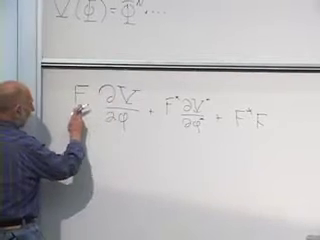
\includegraphics[width=0.82\textwidth]{lecture_09_figure_04.png}
\lectureframe{00:39:40.000}
\caption{Biểu thức đầy đủ của trường phụ và phương trình chuyển động đại số của nó, hiện ra cùng nhau sau khi phần che khuất trên bảng được gỡ bỏ.}
\end{figure}

\begin{classroomqa}
\audiencequestion{Có phải đạo hàm đó nên được lấy theo \(\phi\), thay vì theo trường liên hợp được viết trên bảng không? \lecturetimestamp{00:41:21}}
\lecturerresponse{Đúng. Sửa lại như vậy sẽ khôi phục cặp liên hợp trong phương trình~\eqref{eq:l9-F-eom}: \(F^\ast=-W'(\phi)\) và \(F=-\overline{W'(\phi)}\).}
\end{classroomqa}

Thế vào phương trình~\eqref{eq:l9-LF} ta được
\begin{equation}
\mathcal L_F\big|_{\mathrm{on\ shell}}
=-|W'(\phi)|^2.
\end{equation}
Vì Lagrangian vô hướng có dạng động năng trừ thế năng, nên thế vô hướng thông thường là
\begin{equation}
\boxed{V(\phi,\phi^\ast)=|W'(\phi)|^2\ge0.}
\label{eq:l9-F-potential}
\end{equation}
\(V\) này không phải là siêu thế. Ta dành \(W\) cho hàm chỉnh hình trên siêu không gian và \(V\) cho thế năng thông thường.

\subsection{Hai ví dụ trực tiếp}

Với các chuẩn hóa quy ước chính xác,
\begin{equation}
\begin{gathered}
W(\Phi)=\frac12m\Phi^2,\\
W'(\phi)=m\phi,
\qquad V=|m|^2|\phi|^2.
\end{gathered}
\label{eq:l9-quadratic-W}
\end{equation}
Cùng hạng đó cho khối lượng fermion \(-\tfrac12m\psi\psi+\mathrm{h.c.}\), nên khối lượng của vô hướng và fermion trùng nhau trước khi siêu đối xứng bị phá vỡ.

Đối với
\begin{equation}
W(\Phi)=\frac{g}{3}\Phi^3,
\end{equation}
ta thu được
\begin{equation}
\begin{gathered}
W'(\phi)=g\phi^2,
\qquad V=|g|^2|\phi|^4,\\
\mathcal L_{\mathrm{Yukawa}}
=-g\phi\psi\psi+\mathrm{h.c.}
\end{gathered}
\label{eq:l9-cubic-W}
\end{equation}
Đỉnh vô hướng bậc bốn mô tả tán xạ hai vô hướng, còn hạng Yukawa là đối tác siêu đối xứng của nó.

\section{Hai loại chân không}

Chân không là một cấu hình trường hằng tại một cực tiểu của \(V\); các hạng đạo hàm của nó triệt tiêu. Vì phương trình~\eqref{eq:l9-F-potential} không âm, nên có thể xảy ra hai trường hợp.

\subsection{Một cực tiểu năng lượng bằng không}

Nếu một \(\phi_0\) nào đó thỏa mãn
\begin{equation}
W'(\phi_0)=0,
\end{equation}
thì
\begin{equation}
V(\phi_0)=0,
\qquad
\langle F\rangle=0.
\label{eq:l9-unbroken-F}
\end{equation}
Chân không là siêu đối xứng. Đây là tương tự của từ độ triệt tiêu: không có thành phần phụ nào chọn ra một phương trong siêu không gian.

\subsection{Một cực tiểu bị nâng lên}

Nếu các phương trình
\begin{equation}
W'(\phi)=0
\label{eq:l9-F-flatness}
\end{equation}
không có nghiệm đồng thời tại cực tiểu, thì
\begin{equation}
V_{\min}>0,
\qquad
\langle F\rangle\neq0,
\label{eq:l9-broken-F}
\end{equation}
và siêu đối xứng bị phá vỡ tự phát. Tác dụng vẫn siêu đối xứng; trạng thái năng lượng thấp nhất của nó thì không.

\begin{figure}[H]
\centering
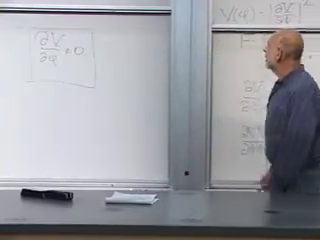
\includegraphics[width=0.88\textwidth]{lecture_09_figure_05.png}
\lectureframe{00:52:09.960}
\caption{Trên bảng vẫn giữ hiện rõ thế dương, phương trình \(F\) và điều kiện chân không, đồng thời phân biệt các phương trình đối xứng với một nghiệm không đối xứng.}
\end{figure}

Phát biểu về tham số trật tự có thể được làm chính xác thông qua phép biến đổi của fermion:
\begin{equation}
\delta\psi_\alpha
=
i\sqrt2
(\sigma^\mu\bar\epsilon)_\alpha\partial_\mu\phi
+\sqrt2\,\epsilon_\alpha F.
\label{eq:l9-fermion-transformation}
\end{equation}
Đối với chân không đồng nhất, hạng đạo hàm triệt tiêu. Nếu
\(\langle F\rangle\neq0\), siêu đối xứng biến đổi fermion bằng cách cộng thêm một hằng khác không, nên chân không không thể bất biến.\editorialnote{Phương trình~\eqref{eq:l9-fermion-transformation} là dạng thành phần chuẩn, làm tường minh phát biểu trong bài giảng rằng các thành phần của siêu trường biến đổi lẫn nhau.}

Cùng kết luận đó cũng suy ra từ siêu đại số. Trong hệ quy chiếu nghỉ,
\begin{equation}
\{Q_\alpha,Q_{\dot\alpha}^\dagger\}
=2\sigma^0_{\alpha\dot\alpha}H.
\end{equation}
Lấy giá trị kỳ vọng chân không biểu diễn năng lượng của nó thành tổng các chuẩn của các siêu điện tích tác dụng lên chân không:
\begin{equation}
E_0\ge0,
\qquad
E_0=0
\ \Longleftrightarrow\
Q_\alpha|0\rangle
=Q_{\dot\alpha}^\dagger|0\rangle=0.
\label{eq:l9-algebra-vacuum-energy}
\end{equation}
Vì vậy, năng lượng chân không dương và sự phá vỡ siêu đối xứng tự phát là hai mặt của cùng một phát biểu về siêu đối xứng cứng.

\begin{center}
\begin{tikzpicture}[x=1.2cm,y=1.0cm,>=Latex]
  \draw[->] (-3,0) -- (-0.2,0) node[right] {\(\phi\)};
  \draw[->] (-2.8,-0.15) -- (-2.8,2.1) node[above] {\(V\)};
  \draw[thick,teal!75!black,domain=-2.5:-0.5,samples=60]
    plot (\x,{0.65*(\x+1.5)^2});
  \fill (-1.5,0) circle (2pt);
  \node[below] at (-1.5,0) {\(F=0\)};
  \draw[->] (0.4,0) -- (3.2,0) node[right] {\(\phi\)};
  \draw[->] (0.6,-0.15) -- (0.6,2.1) node[above] {\(V\)};
  \draw[thick,orange!85!black,domain=0.9:2.9,samples=60]
    plot (\x,{0.55*(\x-1.9)^2+0.65});
  \fill (1.9,0.65) circle (2pt);
  \draw[dashed] (0.6,0.65) -- (1.9,0.65);
  \node[below] at (1.9,0.65) {\(F\neq0\)};
\end{tikzpicture}
\end{center}

\editorialnote{Một minh họa tối thiểu là \(W=f\Phi\), với trường hợp đó \(W'=f\) không bao giờ triệt tiêu và \(V=|f|^2\). Ví dụ một trường ấy có một phương vô hướng phẳng; sự phá vỡ \(F\)-term ổn định, thực tế, thường được thực hiện với nhiều trường chiral, như trong các vùng ẩn kiểu O'Raifeartaigh.}

\section{Sự phá vỡ siêu đối xứng tạo ra gì}

\subsection{Phân tách khối lượng}

Phép tương tự với sắt từ giờ lại quay về phổ năng lượng. Một từ trường nội yếu tách các mức nguyên tử mà không phá hủy bản sắc của nguyên tử. Tương tự, một tham số trật tự phá vỡ siêu đối xứng được truyền yếu sẽ tách các boson và fermion mà nếu không thì sẽ cùng nằm trong một siêu đa bội.

\begin{classroomqa}
\audiencequestion{Những hạt nào được siêu đối xứng biến đổi lẫn nhau và vì thế mất sự suy biến khối lượng khi chân không phá vỡ nó? \lecturetimestamp{00:51:40}}
\lecturerresponse{Boson và fermion. Khối lượng của chúng không nhất thiết còn bằng nhau một khi trạng thái không còn tôn trọng phép biến đổi liên hệ chúng.}
\end{classroomqa}

Sự phân tách không do \(\langle F\rangle\) tự nó tạo ra; nó phụ thuộc vào các tương tác truyền sự phá vỡ tới các trường khả kiến. Nếu các tương tác đó yếu, các hạt khả kiến vẫn còn nhận ra được và các độ phân tách nhỏ so với các thang thống nhất lớn hoặc Planck. Nếu chúng mạnh, phép tương tự sẽ là một nguyên tử bị bóp méo bởi một từ trường khổng lồ đến mức trở thành một vật dài, không còn nhận ra được.

\subsection{Goldstino}

Đối với một bộ sinh bị phá vỡ thông thường, \(J|0\rangle\) cho một trạng thái Goldstone boson. Một siêu điện tích có tính fermion và biến các trạng thái boson thành các trạng thái fermion. Vì chân không được tính là boson, một siêu điện tích bị phá vỡ tạo ra một trạng thái fermion năng lượng bằng không:
\begin{equation}
Q_\alpha|0\rangle
\sim
|\widetilde G_\alpha,\mathbf k=0\rangle.
\label{eq:l9-goldstino}
\end{equation}
Trạng thái lan truyền tương ứng của nó là một fermion Weyl không khối lượng, Goldstone fermion hay goldstino.

\begin{classroomqa}
\audiencequestion{Nếu một phép biến đổi siêu đối xứng không giữ chân không cố định, nó tạo ra trạng thái mới nào? \lecturetimestamp{00:53:24}}
\lecturerresponse{Một fermion không khối lượng. Mô thức thông thường của định lý Goldstone vẫn giữ nguyên, nhưng một bộ sinh fermion biến chân không boson thành goldstino.}
\end{classroomqa}

Do đó, sự phá vỡ siêu đối xứng tự phát cứng có hai dấu hiệu không thể tránh khỏi:
\begin{equation}
\boxed{
V_{\min}>0
\qquad\text{and}\qquad
\text{a massless goldstino}.
}
\label{eq:l9-rigid-breaking-signatures}
\end{equation}

\section{Khu vực ẩn}

Thật tiện khi gọi nguyên tử và vật sắt từ là hai khu vực. Vật sắt từ hình thành tham số trật tự; nguyên tử chỉ cảm nhận trường được truyền từ đó. Khi tương tác ghép yếu, thao tác lên nguyên tử hầu như không kích thích một magnon và hầu như không cho khả năng tiếp cận trực tiếp với môi trường từ. Khi ấy vật sắt từ là ẩn, dù sự hiện diện của nó được suy ra từ những phân tách nhỏ trong phổ.

Xây dựng mô hình siêu đối xứng dùng cùng ngôn ngữ ấy. Các trường bổ sung trong một khu vực ẩn có các giá trị kỳ vọng của hạng \(F\) hoặc \(D\) khác không. Các tương tác gọi là cơ chế truyền đạt chuyển sự phá vỡ ấy sang khu vực khả kiến và sinh ra các khối lượng mềm cho các siêu đối tác. Sự truyền yếu giải thích vì sao lý thuyết khả kiến có thể vẫn gần đúng siêu đối xứng ở một thang cơ bản cao hơn nhiều, đồng thời không biểu lộ sự suy biến boson--fermion chính xác ở năng lượng thấp.

Cấu trúc này không tự động. Cần có các trường bổ sung, một chân không phá vỡ ổn định và một cơ chế truyền đạt được kiểm soát. Đó là vì sao bài giảng mô tả sự phá vỡ siêu đối xứng thực tế là phức tạp và phần nào gượng ép, chứ không phải là một hệ quả duy nhất tất yếu của mô hình tối thiểu.

\section{Hấp dẫn làm thay đổi cả hai dấu hiệu}

\subsection{Năng lượng chân không trở thành một nguồn}

Không có hấp dẫn, việc tịnh tiến mọi năng lượng thêm một hằng số không làm thay đổi các thí nghiệm phi hấp dẫn. Có hấp dẫn, mật độ năng lượng chân không đi vào phương trình Einstein như một hằng số vũ trụ. Một \(V_{\min}\) dương gây ra sự giãn nở gia tốc. Nếu thang của nó so sánh được với thang vật lý hạt cần cho khối lượng các siêu đối tác, độ cong thu được sẽ lớn hơn quan sát một cách khổng lồ.

\begin{classroomqa}
\audiencequestion{Một năng lượng chân không dương khác không tác động lên thế giới như thế nào một khi tính đến hấp dẫn? \lecturetimestamp{01:00:40}}
\lecturerresponse{Nó đóng vai trò như một hằng số vũ trụ và gây ra sự giãn nở gia tốc. Ở các thang vật lý hạt thông thường, hiệu ứng đó sẽ lớn đến mức không thể chấp nhận được.}
\end{classroomqa}

Siêu đối xứng địa phương, hay siêu hấp dẫn, làm thay đổi công thức bình phương dương. Để định hướng, thế \(F\)-term chuẩn \(N=1\) là
\begin{equation}
\begin{aligned}
V_F={}&e^{K/M_P^2}
\left(
K^{i\bar j}D_iW\,D_{\bar j}\overline W
-\frac{3|W|^2}{M_P^2}
\right),\\
D_iW={}&\partial_iW+\frac{\partial_iK}{M_P^2}W.
\end{aligned}
\label{eq:l9-sugra-potential}
\end{equation}
Do có hạng âm, năng lượng dương từ sự phá vỡ siêu đối xứng, về nguyên tắc, có thể bị khử một phần. Phần còn lại có thể là một hằng số vũ trụ nhỏ.

\editorialnote{Bài giảng chủ ý chỉ nêu một hiệu chỉnh có tính sơ đồ và nêu rõ sự phân vân về chỗ đặt khối lượng Planck. Phương trình~\eqref{eq:l9-sugra-potential} ghi lại công thức quy ước cho các đa bội chiral với thế Kähler \(K\); các \(D\)-term gauge sẽ thêm một đóng góp không âm nữa. Nó không giải thích giá trị nhỏ xíu được quan sát, điều vẫn là bài toán hằng số vũ trụ.}

\subsection{Cơ chế siêu-Higgs}

Hiệu ứng hấp dẫn thứ hai dễ hiểu nhất nếu đếm các phân cực. Một hạt có khối lượng spin-\(j\) có \(2j+1\) trạng thái spin trong hệ quy chiếu nghỉ của nó.

\begin{classroomqa}
\audiencequestion{Một hạt có khối lượng spin-\(j\) có bao nhiêu trạng thái spin? \lecturetimestamp{01:05:16}}
\lecturerresponse{\(2j+1\). Cụ thể, một hạt spin một có khối lượng có ba trạng thái, trong khi một boson gauge không khối lượng chỉ có các helicity \(+1\) và \(-1\).}
\end{classroomqa}

Sự khác biệt này là thuần động học. Một hạt có khối lượng có thể được boost về nghỉ, rồi được boost theo một hướng mới trong khi định hướng spin của nó vẫn được giữ, nên mọi hình chiếu đều phải tồn tại. Một hạt không khối lượng không thể bị vượt qua hoặc đưa về nghỉ. Do đó nó chỉ có thể mang hai helicity cực trị.

Đối với trường gauge điện yếu,
\begin{equation}
\underbrace{(+1,-1)}_{\text{massless vector}}
+
\underbrace{(0)}_{\text{Goldstone}}
\longrightarrow
\underbrace{(+1,0,-1)}_{\text{massive vector}}.
\label{eq:l9-higgs-count}
\end{equation}

\begin{classroomqa}
\audiencequestion{Phân cực dọc của một \(W\) hoặc \(Z\) có khối lượng đến từ đâu? \lecturetimestamp{01:08:50}}
\lecturerresponse{Từ boson Goldstone. Nó bị hấp thụ bởi trường gauge và hoàn tất biểu diễn spin một có khối lượng với ba trạng thái.}
\end{classroomqa}

Hấp dẫn có graviton không khối lượng spin hai. Đối tác siêu đối xứng của nó là gravitino không khối lượng spin-\(\tfrac32\).

\begin{classroomqa}
\audiencequestion{Spin của graviton là gì, và vì thế spin của siêu đối tác của nó là gì? \lecturetimestamp{01:10:24}}
\lecturerresponse{Graviton có spin \(2\); đối tác fermion lệch đi một nửa đơn vị và có spin \(3/2\).}
\end{classroomqa}

Một gravitino không khối lượng có các helicity \(\pm\tfrac32\), còn một gravitino có khối lượng còn phải có cả \(\pm\tfrac12\). Goldstino cung cấp chính xác các trạng thái còn thiếu ấy:
\begin{equation}
\begin{gathered}
\underbrace{\left(+\frac32,-\frac32\right)}_{\text{massless gravitino}}
\oplus
\underbrace{\left(+\frac12,-\frac12\right)}_{\text{goldstino}}\\
\Downarrow\\
\underbrace{\left(+\frac32,+\frac12,-\frac12,-\frac32\right)}_{\text{massive gravitino}}.
\end{gathered}
\label{eq:l9-super-higgs}
\end{equation}
Đây là cơ chế siêu-Higgs. Một khi siêu đối xứng là địa phương, goldstino bị hấp thụ và không còn xuất hiện như một hạt không khối lượng độc lập. Gravitino thu được tương tác hấp dẫn và vì vậy khó tạo ra.

\section{Chuyển chủ đề: vì sao \texorpdfstring{\(SU(5)\)}{SU(5)}?}

Hình thức luận siêu đối xứng giờ nhường chỗ cho thống nhất lớn. Nhóm gauge của Mô hình Chuẩn là
\begin{equation}
G_{\mathrm{SM}}
=SU(3)_c\times SU(2)_L\times U(1)_Y.
\label{eq:l9-sm-group}
\end{equation}
Ba thừa số của nó lần lượt tổ chức màu, isospin yếu và siêu điện tích yếu. Câu hỏi thống nhất là liệu tích này có phải là nhóm con còn lại của một nhóm đơn lớn hơn hay không, để các đa bội hạt và các lực gauge có vẻ tách biệt thực ra là những phần của một cấu trúc duy nhất. Ứng viên tối thiểu được phát triển ở đây là \(SU(5)\).

\subsection{Các phần tử nhóm và các bộ sinh}

Đối với \(U\in SU(N)\),
\begin{equation}
U^\dagger U=\mathbf1,
\qquad
\det U=1.
\label{eq:l9-SUN-def}
\end{equation}
Điều kiện thứ nhất là tính unitarity; điều kiện thứ hai chính là ý nghĩa của tính đặc biệt. Viết một phần tử vô cùng bé dưới dạng
\begin{equation}
U=\mathbf1+i\epsilon G+\mathcal O(\epsilon^2).
\label{eq:l9-infinitesimal-U}
\end{equation}
Tính unitarity đòi hỏi
\begin{equation}
G^\dagger=G,
\end{equation}
và
\begin{equation}
\det e^{i\epsilon G}
=e^{i\epsilon\operatorname{tr}G}=1
\end{equation}
đòi hỏi
\begin{equation}
\operatorname{tr}G=0.
\end{equation}
Vì vậy, các bộ sinh là các ma trận Hermite vết bằng không.

Một ma trận Hermite \(N\times N\) chứa \(N^2\) tham số thực: \(N\) phần tử chéo thực và \(N(N-1)/2\) phần tử ngoài đường chéo phức. Điều kiện vết bằng không loại đi một tham số. Do đó
\begin{equation}
\dim SU(N)=N^2-1,
\qquad
\dim SU(5)=24.
\label{eq:l9-SU5-dimension}
\end{equation}
Để so sánh, \(SU(2)\) có ba bộ sinh Pauli và \(SU(3)\) có tám bộ sinh màu.

\section{Các khối của Mô hình Chuẩn bên trong \texorpdfstring{\(SU(5)\)}{SU(5)}}

Tách không gian năm chiều thành một khối yếu hai chiều và một khối màu ba chiều:
\begin{equation}
\mathbf5=\mathbf2\oplus\mathbf3.
\end{equation}
Các bộ sinh được nhúng có dạng
\begin{align}
T^a_L
&=
\begin{pmatrix}
\tfrac12\tau^a&0\\
0&0_{3\times3}
\end{pmatrix},
&& a=1,2,3,
\label{eq:l9-SU2-block}\\
T^A_c
&=
\begin{pmatrix}
0_{2\times2}&0\\
0&\tfrac12\lambda^A
\end{pmatrix},
&& A=1,\ldots,8.
\label{eq:l9-SU3-block}
\end{align}
Các ma trận Pauli \(\tau^a\) sinh ra \(SU(2)\) yếu; các ma trận Gell-Mann \(\lambda^A\) sinh ra \(SU(3)\) màu. Vì các khối không chồng lấn lên nhau, hai nhóm con giao hoán.

Một bộ sinh chéo bổ sung nữa tỷ lệ với ma trận đơn vị trong mỗi khối và vì thế giao hoán với cả hai. Trong biểu diễn cơ bản, một quy ước siêu điện tích gấp đôi thuận tiện là
\begin{equation}
T_Y^{(\mathbf5)}=
\operatorname{diag}
\left(
1,1,-\frac23,-\frac23,-\frac23
\right).
\label{eq:l9-hypercharge-generator}
\end{equation}
Vết của nó triệt tiêu:
\begin{equation}
1+1-3\left(\frac23\right)=0.
\end{equation}
Biểu diễn vật chất liên hợp có các trị riêng đối dấu,
\begin{equation}
Y_{\overline{\mathbf5}}
=
\operatorname{diag}
\left(
-1,-1,\frac23,\frac23,\frac23
\right),
\label{eq:l9-fivebar-hypercharge}
\end{equation}
đó là các giá trị được viết cho cột vật chất trong bài giảng. Dấu tổng thể và chuẩn hóa là theo quy ước; các mục này dùng quy ước của Mô hình Chuẩn
\begin{equation}
Q=T_3+\frac{Y}{2}.
\label{eq:l9-charge}
\end{equation}
Các phương trình~\eqref{eq:l9-SU2-block}--\eqref{eq:l9-hypercharge-generator} cho thấy
\begin{equation}
SU(3)_c\times SU(2)_L\times U(1)_Y
\subset SU(5).
\end{equation}

Ba bộ sinh yếu, tám bộ sinh màu và một bộ sinh siêu tích chiếm \(12\) trong số \(24\) bộ sinh \(SU(5)\).\editorialnote{Mười hai bộ sinh còn lại nằm trong các khối ngoài đường chéo \(2\times3\) và \(3\times2\). Các boson gauge của chúng biến các thành phần kiểu quark và kiểu lepton thành lẫn nhau; đây là nguồn gốc về mặt cấu trúc của các tương tác làm biến đổi baryon và lepton sẽ được triển khai ở phần tiếp theo.}

\begin{classroomqa}
\audiencequestion{Những hạt chuẩn nào tương ứng với các bộ sinh của các phân nhóm quen thuộc? \lecturetimestamp{01:31:05}}
\lecturerresponse{Tám bộ sinh \(SU(3)\) cho tám gluon. Ba bộ sinh \(SU(2)\) cho các trường gauge yếu, sau khi trộn điện-yếu thì trở thành \(W^\pm\) và một phần của hệ \(Z\)-phôtôn; trường \(U(1)\) cung cấp tổ hợp trung hòa còn lại.}
\end{classroomqa}

\section{Một họ trong ngôn ngữ tay trái}

Tập trung vào thế hệ thứ nhất; cùng một khuôn mẫu lặp lại cho các thế hệ muon/charm/strange và tau/top/bottom. Cách tiết kiệm nhất là đếm mọi trường Weyl độc lập như đều là tay trái. Các hạt tay phải được biểu diễn bằng các trường liên hợp điện tích tay trái của chúng:
\begin{equation}
Q_L=(u_L,d_L),\quad
L_L=(\nu_{eL},e_L),\quad
u^c_L,\quad d^c_L,\quad e^c_L.
\end{equation}
Số lượng tương ứng là
\begin{equation}
\underbrace{6}_{Q_L}
+
\underbrace{2}_{L_L}
+
\underbrace{3}_{u^c_L}
+
\underbrace{3}_{d^c_L}
+
\underbrace{1}_{e^c_L}
=15.
\label{eq:l9-fifteen-fields}
\end{equation}

\editorialnote{Mô hình Chuẩn tối thiểu không chứa trường Weyl neutrino tay phải độc lập nào, nên số đếm là \(15\). Riêng phép đếm này không khẳng định neutrino là một hạt Majorana. Thêm một singlet \(\nu^c_L\) đưa tổng số lên \(16\) trường và tự nhiên dẫn tới \(SO(10)\), vượt ra ngoài phép xây dựng \(SU(5)\) hiện tại.}

Đa bội năm chiều phải đặt các thành phần bộ đôi yếu không màu vào hai vị trí đầu và các singlet yếu mang màu vào ba vị trí cuối.

\begin{classroomqa}
\audiencequestion{Cột được đề xuất có sáu trường chứ không phải năm sao? \lecturetimestamp{01:36:14}}
\lecturerresponse{Không. Quark up đã được viết ra trong lượt đầu tiên bị xóa đi. Cột đó là neutrino, electron và ba bản sao màu của phản quark down: tổng cộng là năm thành phần.}
\end{classroomqa}

Khi đó ta được
\begin{equation}
\overline{\mathbf5}
=
\begin{pmatrix}
\nu_{eL}\\
e_L\\
d^c_{rL}\\
d^c_{gL}\\
d^c_{bL}
\end{pmatrix}.
\label{eq:l9-fivebar}
\end{equation}
\editorialnote{Ban đầu bài giảng chỉ gọi đây đơn giản là một đa bội năm chiều. Trong ký hiệu \(SU(5)\) chuẩn, với mọi trường đều viết tay trái, các gán màu và siêu tích của nó xác định nó là biểu diễn liên hợp \(\overline{\mathbf5}\).}
Hai thành phần đầu biến đổi dưới \(SU(2)_L\) nhưng không mang màu. Ba thành phần cuối biến đổi như một phản-bộ ba dưới đối xứng màu nhưng là các singlet yếu.

\begin{classroomqa}
\audiencequestion{Những quark nào mang màu nhưng không mang số lượng tử \(SU(2)_L\), khi mọi trường đều được viết tay trái? \lecturetimestamp{01:40:13}}
\lecturerresponse{Các liên hợp điện tích của các quark tay phải. Với đa bội năm thành phần này, phép kiểm tra điện tích chọn ra ba trường phản quark down \(d^c_{r,g,b}\).}
\end{classroomqa}

Các điện tích trong phương trình~\eqref{eq:l9-fivebar} có tổng bằng 0:
\begin{equation}
0-1+\frac13+\frac13+\frac13=0.
\label{eq:l9-fivebar-charge-sum}
\end{equation}
Điều đó là bắt buộc vì toán tử điện tích là một tổ hợp không vết của các bộ sinh \(SU(5)\).

\begin{classroomqa}
\audiencequestion{Tại sao các phản quark down, chứ không phải các phản quark up, chiếm ba vị trí màu? \lecturetimestamp{01:43:38}}
\lecturerresponse{Neutrino và electron đóng góp tổng điện tích \(-1\). Ba màu của phản quark down đóng góp \(+1\), làm cho vết bằng 0. Ba trường phản-up sẽ cho tổng điện tích sai.}
\end{classroomqa}

Mười trường tay trái còn lại là
\begin{equation}
Q_L\;(6)
\oplus
u^c_L\;(3)
\oplus
e^c_L\;(1),
\end{equation}
và chúng khớp chính xác với biểu diễn phản đối xứng hạng hai
\begin{equation}
\mathbf{10}\cong\wedge^2\mathbf5,
\qquad
\dim\wedge^2\mathbf5=\binom52=10.
\label{eq:l9-ten-preview}
\end{equation}
Việc sắp xếp tường minh của chúng là nhiệm vụ của bài giảng tiếp theo. Sự khớp về số lượng
\begin{equation}
\overline{\mathbf5}\oplus\mathbf{10}
\end{equation}
cho mỗi họ của Mô hình Chuẩn là bằng chứng nổi bật đầu tiên cho thấy ý tưởng \(SU(5)\) không chỉ là một cách gán nhãn lại tùy ý.

\begin{classroomqa}
\audiencequestion{Nếu bộ năm và bộ mười là các biểu diễn khác nhau, điều đó có nghĩa là các hạt của chúng không thể tương tác với nhau sao? \lecturetimestamp{01:46:14}}
\lecturerresponse{Không. Một phép biến đổi nhóm tác dụng bên trong từng biểu diễn bất khả quy, nên nó không trực tiếp biến một phần tử của bộ năm thành một phần tử của bộ mười. Tuy vậy, hai tập đó vẫn có thể tương tác bằng cách phát và hấp thụ các boson gauge chung, và các ghép nối Higgs cũng có thể nối các trường của chúng.}
\end{classroomqa}

\section{Toàn cảnh}

Bài giảng đã lần theo một khuôn mẫu xuyên suốt những thang đo rất khác nhau. Bất biến quay làm cho các mức nguyên tử suy biến; một nền từ trường tách chúng ra. Một chất sắt từ tạo ra nền như vậy trong khi các định luật cơ sở vẫn đối xứng, và các magnon không khe năng lượng của nó cho thấy sự bất đối xứng nằm ở chân không. Trong một lý thuyết siêu đối xứng chiral, giá trị kỳ vọng của trường phụ trợ đóng vai trò tham số trật tự:
\begin{equation}
\begin{aligned}
\langle F\rangle=0
&\quad\Longleftrightarrow\quad
\text{unbroken supersymmetry},\\
\langle F\rangle\neq0
&\quad\Longrightarrow\quad
\text{spontaneous breaking}.
\end{aligned}
\end{equation}
Chân không bị phá vỡ mang năng lượng dương trong siêu đối xứng cứng, tách các siêu đa bội và tạo ra một goldstino. Sự trung gian yếu gợi ý một sector ẩn; hấp dẫn biến năng lượng chân không thành một vấn đề vũ trụ học và hấp thụ goldstino vào một gravitino có khối lượng.

Phép xây dựng \(SU(5)\) ở phần kết mở ra một câu hỏi mới chứ không hoàn tất nó. Các bộ sinh \(5\times5\) Hermite không vết chứa các khối của Mô hình Chuẩn, và năm trường vật chất đầu tiên khớp chính xác dưới dạng \((\nu_e,e^-,d^c_r,d^c_g,d^c_b)\). Mười trường còn lại đang chờ trong biểu diễn phản đối xứng. Chính sự khớp còn dang dở đó là nơi sự thống nhất lớn thật sự bắt đầu.
